\chapter{Numerical Examples: ERT-Conditioned Material Fields}
\label{chap:inversion-results}

\section{Purpose and Scope}
\label{sec:inversion-purpose}

\revadd{17}{This chapter records the numerical examples that have now been run
for the CD-A Niche 4 ERT problem.}{\annCommentSeventeen}  It is intentionally an
ERT chapter.  The model equations, boundary conditions, and measurement inventory
remain those of Chapters~\ref{chap:ogs-model} and~\ref{chap:measurements}; the
results here test how far the ERT support data can be matched by changing a small
set of material-field and observation-model parameters.

Three messages are carried forward.  First, the ERT comparison prefers a time
shift of about three months relative to the OGS time origin, while the active
open-niche seasonal boundary curve is not shifted in the model input.  Second, a
single global Archie law does not fit the ERT supports as well as support-wise
Archie calibration.  Third, the current successful ERT parameterisation uses a
permeability-magnitude random field and a porosity random field.  The tensor shape
is still controlled by scalar angle and ratio parameters; the available results do
not show that releasing a fully spatial tensor field is the missing step.

\section{Parameterisation and Observation Model}
\label{sec:inversion-modelling-choices}

The permeability field reported in the figures is \(K_{\mathrm{mag}}\), the
first principal intrinsic-permeability value before tensor rotation.  It is not
the determinant, trace, or norm of the tensor.  The random field is represented
as
\begin{equation}
  \log_{10} K_{\mathrm{mag}}(\xx)
  = k_0 + \sum_{j=1}^{100} \xi^K_j \psi_j(\xx),
  \label{eq:permeability-magnitude-rf}
\end{equation}
where \(k_0\) is the global \(\log_{10}\)-permeability level, \(\psi_j\) are
spatial basis functions, and \(\xi^K_j\) are permeability-field coefficients.  The
OGS tensor input \(\KK\) is then reconstructed from \(K_{\mathrm{mag}}\), a
sampled tensor rotation \(\alpha\), and a sampled principal-value ratio
\(q=K_{2}/K_{1}\).  Before rotation, the principal values are
\[
K_{1}(\xx)=K_{\mathrm{mag}}(\xx),
\qquad
K_{2}(\xx)=qK_{\mathrm{mag}}(\xx).
\]
With
\[
R(\alpha)=
\begin{bmatrix}
\cos\alpha & -\sin\alpha\\
\sin\alpha & \cos\alpha
\end{bmatrix},
\]
the cell-wise tensor passed through the OGS \path{k_i_rd} field is
\begin{equation}
  \KK(\xx)=
  R(\alpha)
  \begin{bmatrix}
  K_{\mathrm{mag}}(\xx) & 0\\
  0 & q\,K_{\mathrm{mag}}(\xx)
  \end{bmatrix}
  R(\alpha)^{T}.
  \label{eq:permeability-ratio-angle-tensor}
\end{equation}
Equivalently, the tensor components written to OGS are
\begin{align}
  K_{11} &= K_{\mathrm{mag}}(\cos^2\alpha + q\sin^2\alpha), \\
  K_{22} &= K_{\mathrm{mag}}(\sin^2\alpha + q\cos^2\alpha), \\
  K_{12} &= K_{21}
  = K_{\mathrm{mag}}(1-q)\sin\alpha\cos\alpha .
  \label{eq:permeability-tensor-components}
\end{align}
If the same tensor is written with geometric-mean magnitude \(k_g(\xx)\) and
anisotropy ratio \(r=K_{1}/K_{2}\), then
\(k_g=K_{\mathrm{mag}}\sqrt{q}\), \(r=1/q\), and
\(\KK=R(\alpha)\operatorname{diag}(k_g\sqrt r,k_g/\sqrt r)R(\alpha)^T\).

The porosity field uses a bounded 100-mode random field around a sampled mean:
\begin{align}
  d_{\por}(\xx) &= \sum_{\ell=1}^{100}\eta_\ell\varphi_\ell(\xx),\\
  \por(\xx) &= \por_{\min}
  + \frac{\por_{\max}-\por_{\min}}
  {1+\exp[-\{\beta_{\por}+1.25(d_{\por}(\xx)-\overline{d_{\por}})\}]},
  \label{eq:porosity-kl-field}
\end{align}
where \(\eta_\ell\) are porosity-field coefficients, \(\varphi_\ell\) are the
spatial basis functions, \(\overline{d_{\por}}\) is the mesh mean of
\(d_{\por}\), \(\por_{\min}=0.05\), \(\por_{\max}=0.175\), and
\(\beta_{\por}\) is chosen so that the mesh mean equals the sampled mean porosity
\(\phi_0\).

The sampled material state is therefore not a fully free tensor field.  For
permeability, \(K_{\mathrm{mag}}\) is spatially random through \(k_0\) and
\(\xi^K_j\), while \(\alpha\) and \(q\) are random scalar controls shared by the
mesh.  For porosity, \(\phi_0\) is a random scalar mean and \(\eta_\ell\) are the
spatial random-field coefficients.  Table~\ref{tab:inversion-parameter-bookkeeping}
also lists the fixed boundary controls and fitted observation-model coefficients.

\begingroup
\small
\setlength{\tabcolsep}{3pt}
\renewcommand{\arraystretch}{1.12}
\begin{center}
\captionof{table}{Prior coordinates and fixed controls used by the current
ERT-conditioned examples.}
\label{tab:inversion-parameter-bookkeeping}
\begin{tabular}{@{}L{0.24\textwidth} L{0.33\textwidth} L{0.33\textwidth}@{}}
\toprule
Coordinate & Status and prior or treatment & Short role\\
\midrule
\(k_0\) & sampled; \(\mathcal N(-21.02,5.1^2)\) &
Global level in Eq.~\eqref{eq:permeability-magnitude-rf}.\\
\(\xi^K_1,\ldots,\xi^K_{100}\) & sampled; independent \(\mathcal N(0,1)\) &
Permeability-magnitude random-field coefficients.\\
\(\alpha\) & sampled; \(\mathcal N(139.9,5^2)\), bounded to
\(0\)--\(180^\circ\) &
Rotation in Eq.~\eqref{eq:permeability-ratio-angle-tensor}.\\
\(\log_{10}q\) & sampled; \(\mathcal N(\log_{10}0.45,0.30^2)\), bounded by
\(\log_{10}[0.1,0.9]\) &
Tensor ratio in Eq.~\eqref{eq:permeability-ratio-angle-tensor}.\\
\(\phi_0\) & sampled; truncated \(\mathcal N(0.1504,0.012^2)\) on
\(0.05\)--\(0.175\) &
Mean target for Eq.~\eqref{eq:porosity-kl-field}.\\
\(\eta_1,\ldots,\eta_{100}\) & sampled; independent \(\mathcal N(0,1)\) &
Porosity random-field coefficients.\\
\(\Delta t_{\mathrm{ERT}}\) & sampled; truncated \(\mathcal N(96.082,10^2)\) d on
\(66.082\)--\(106.082\) d &
ERT observation-time alignment.\\
\(\Delta t_{\mathrm{niche}},s_{\mathrm{niche}},c_{\mathrm{niche}}\) &
fixed to \(0\) d, \(1\), and \(0\) MPa in this run &
Open-niche suction-curve shift, scale, and offset.\\
\(a_s,b_s\) & fitted per support, not sampled; \(a_s\in[-0.7,1.3]\),
\(b_s\in[-2.0,-0.2]\) &
Local Archie intercept and slope in Eq.~\eqref{eq:local-archie}.\\
\bottomrule
\end{tabular}
\end{center}
\endgroup

For each ERT support \(s\) and time \(t_j\), let \(y_{s,j}\) be measured
\(\log_{10}\)-resistivity and \(h_s(t_j;\vartheta)\) the support response from
OGS or the trained surrogate for a parameter vector \(\vartheta\).  Two Archie
observation models are compared:
\begin{align}
  \widehat{y}_{s,j} &= a_s + b_s\,h_s(t_j;\vartheta)
  &&\text{support-wise, or local, Archie}, \label{eq:local-archie}\\
  \widehat{y}_{s,j} &= a + b\,h_s(t_j;\vartheta)
  &&\text{global Archie}. \label{eq:global-archie}
\end{align}
The local model is flexible because every support has its own intercept and
slope.  The global model is the stricter test: one electrical calibration must
explain all 20 support curves.

\section{Time Alignment}
\label{sec:inversion-time-alignment}

Figure~\ref{fig:numerical-ert-time-shift} shows the posterior distribution of the
ERT time shift.  The posterior median is \(93.3\) d and the 5--95\% interval is
\(78.9\)--\(104.3\) d.  The best-likelihood retained sample is close to
\(96.1\) d.  This is not a material parameter: it says that the ERT observation
time axis is displaced relative to the OGS time origin.  Because the active
open-niche boundary curve is fixed at zero shift in these examples, the ERT
responses and the seasonal boundary forcing should not be read as already
time-consistent.

\begin{figure}[htbp]
  \centering
  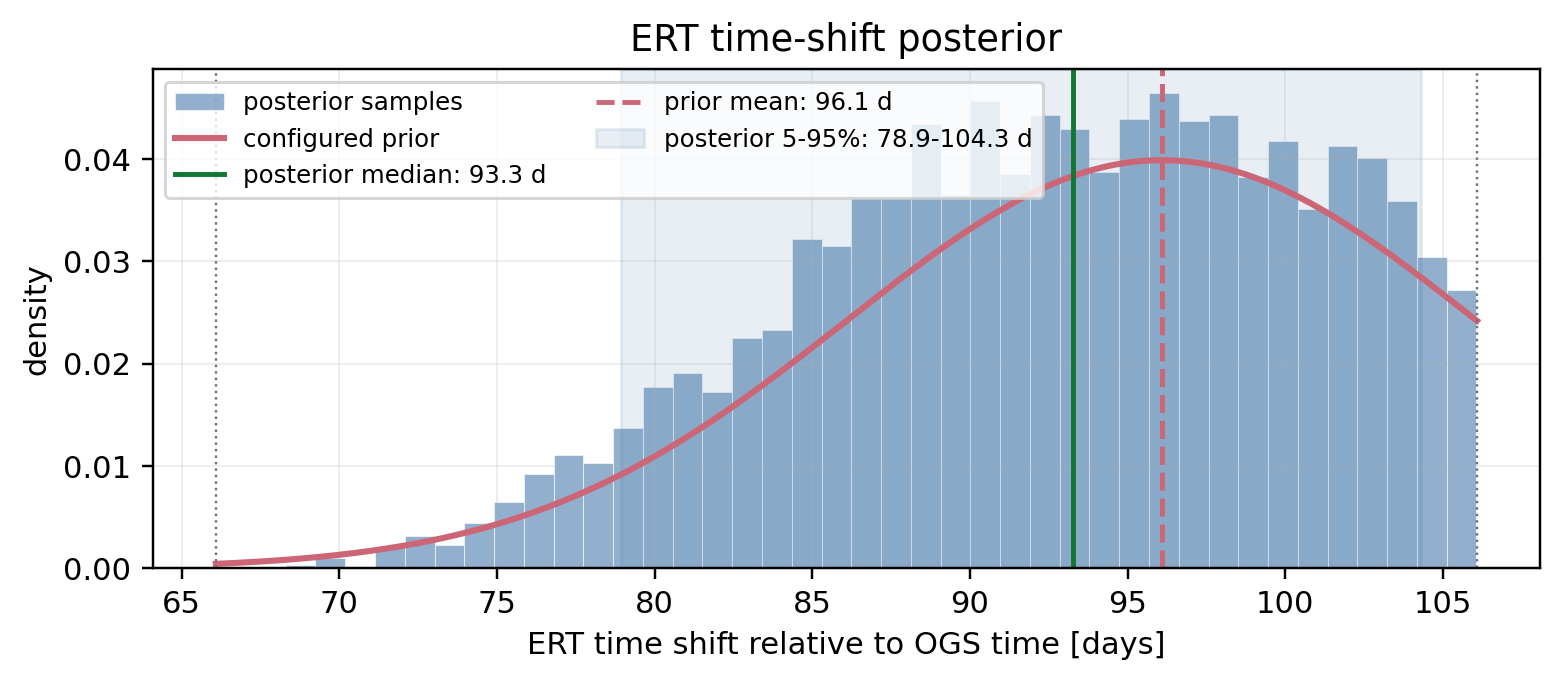
\includegraphics[width=0.86\textwidth]{resources/figures/numerical_ert_time_shift_distribution.png}
  \caption{Posterior distribution of the ERT time-shift parameter.  The configured
  prior is shown with the retained posterior samples; the posterior remains centred
  near a three-month shift.}
  \label{fig:numerical-ert-time-shift}
\end{figure}

\FloatBarrier

\section{Local and Global Archie}
\label{sec:inversion-local-global-archie}

The strongest current ERT fits use local Archie calibration.  In the retained
raw-\(\log_{10}\) posterior, the best-likelihood sample has MAE \(0.0241\)
\(\log_{10}\)-resistivity units and the posterior-median fit has mean absolute
median residual \(0.0248\).  The exact local-Archie ERT20 runs give the same
scale of fit: about \(0.024\)--\(0.028\) MAE.  By contrast, the global-Archie
free-\(t_0\) diagnostic did not become a posterior run; its best pre-crash
candidate stays near \(0.0825\) MAE.

\begin{figure}[htbp]
  \centering
  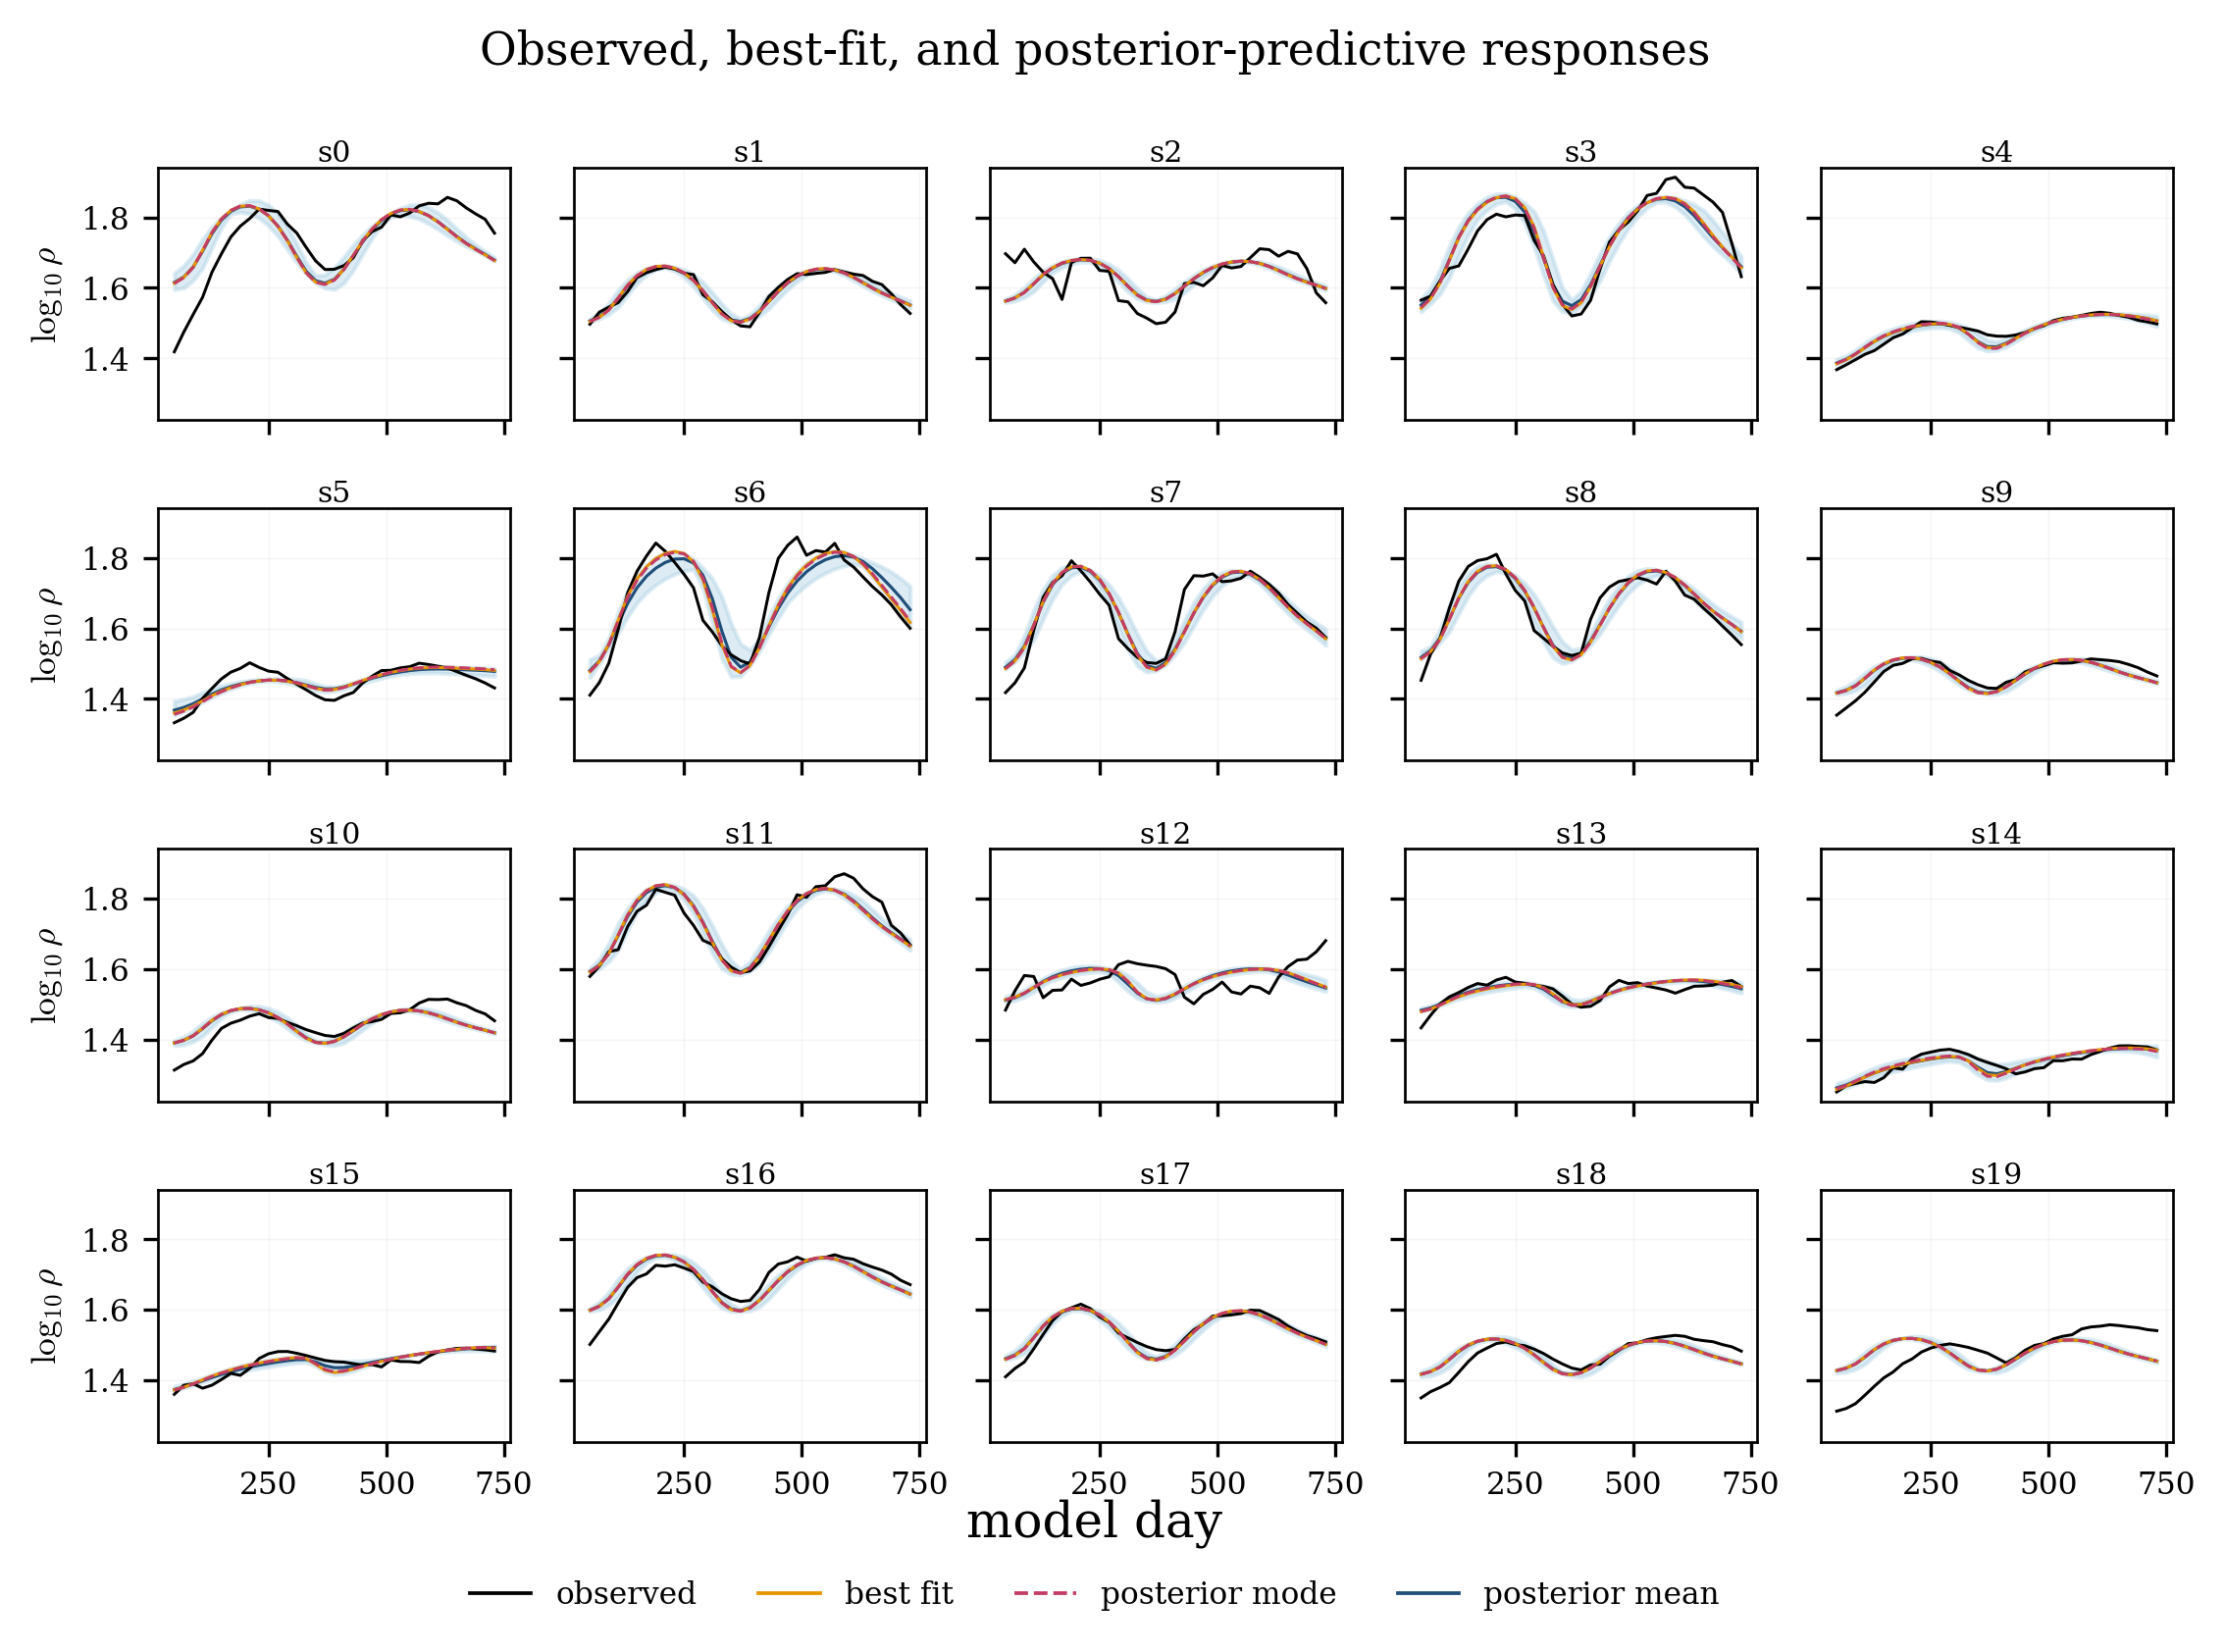
\includegraphics[width=0.98\textwidth]{resources/figures/numerical_local_archie_fit.png}
  \caption{Local-Archie ERT20 fit.  Each ERT support has its own fitted
  \(a_s,b_s\) pair, and the resulting support-wise fit reaches
  \(0.028417\) MAE in the exact exploratory run.}
  \label{fig:numerical-local-archie-fit}
\end{figure}

\begin{figure}[htbp]
  \centering
  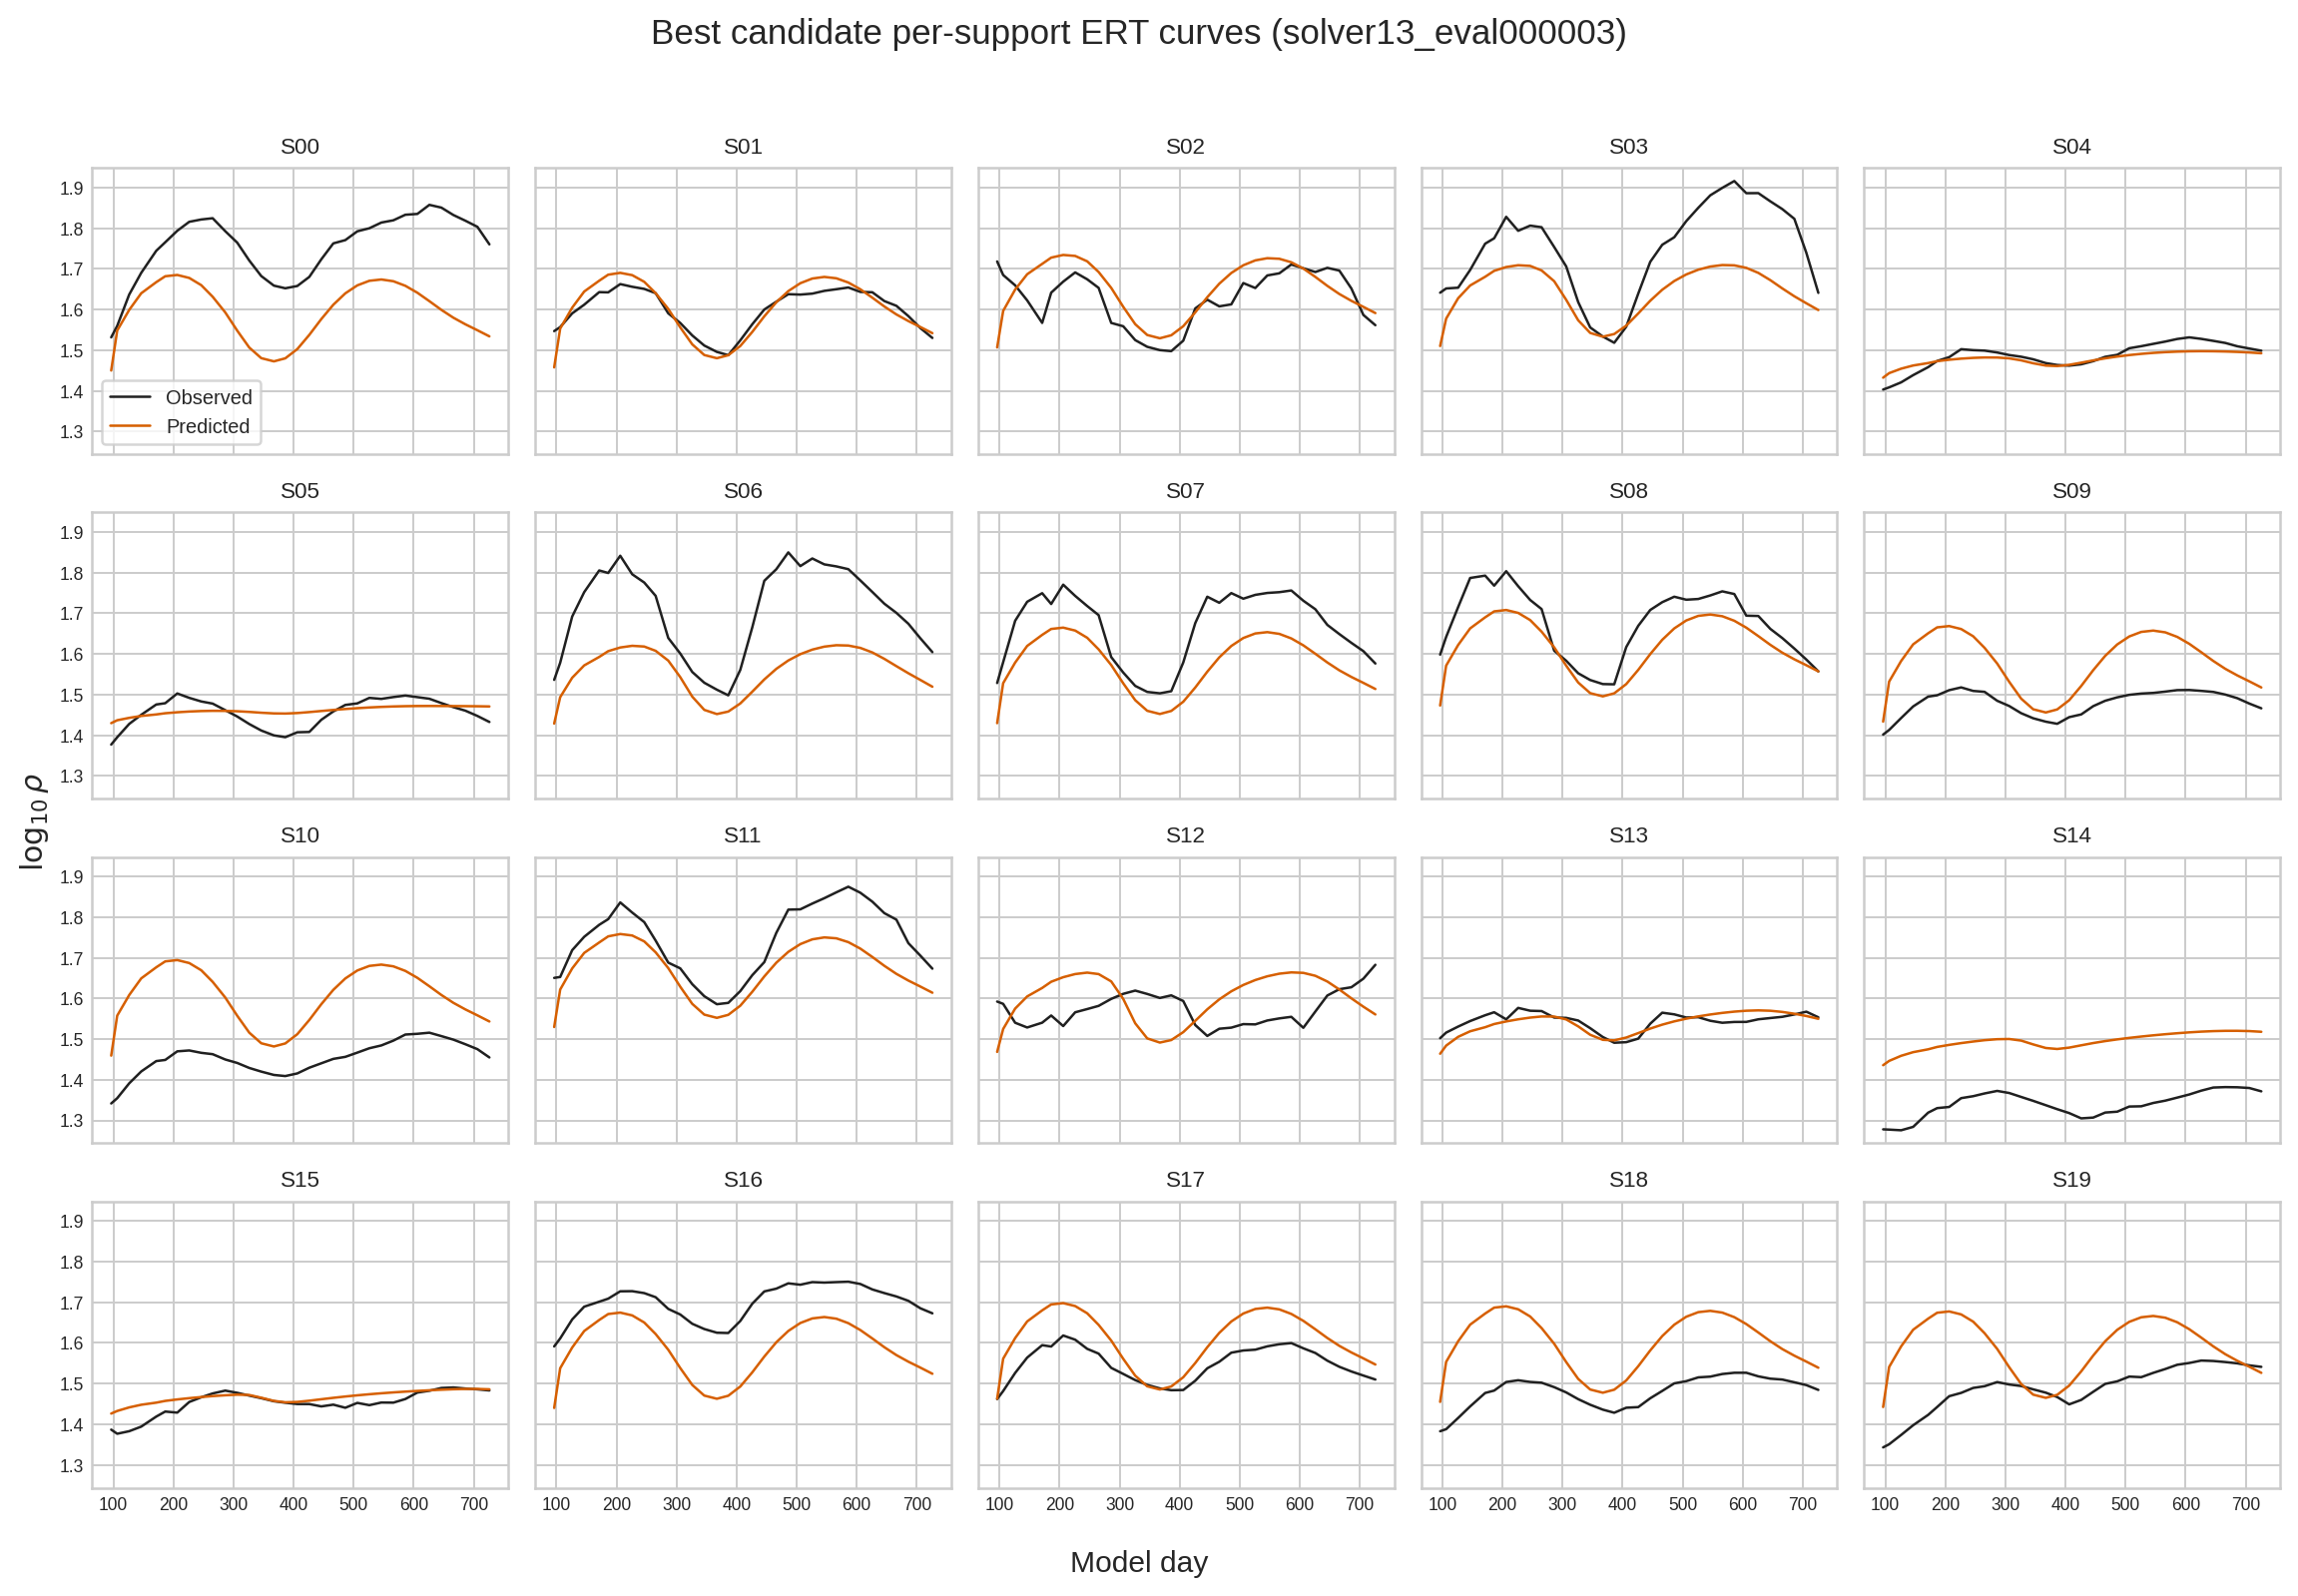
\includegraphics[width=0.98\textwidth]{resources/figures/numerical_global_archie_fit.png}
  \caption{Global-Archie free-\(t_0\) diagnostic.  One \(a,b\) pair is used for all
  supports; the best pre-crash exact candidate has MAE about \(0.0825\).}
  \label{fig:numerical-global-archie-fit}
\end{figure}

\FloatBarrier

The circular Archie summary in
Fig.~\ref{fig:numerical-archie-circular-posterior} explains why this matters.
The fitted coefficients are not just noisy constants: the posterior medians and
5--95\% bands vary by support angle and by the 15 cm versus 30 cm rings.  This
has two possible interpretations.  It may be compensating for an imperfect ERT
support operator, electrode/contact effects, shallow current paths, or electrical
anisotropy not represented in the current observation model.  It may also be a
real indication that the hydraulic-to-electrical mapping is local near the niche.
Either way, the local-Archie residual should not be interpreted as a pure
permeability-field likelihood until the ERT support and electrical model are
settled.

\begin{figure}[htbp]
  \centering
  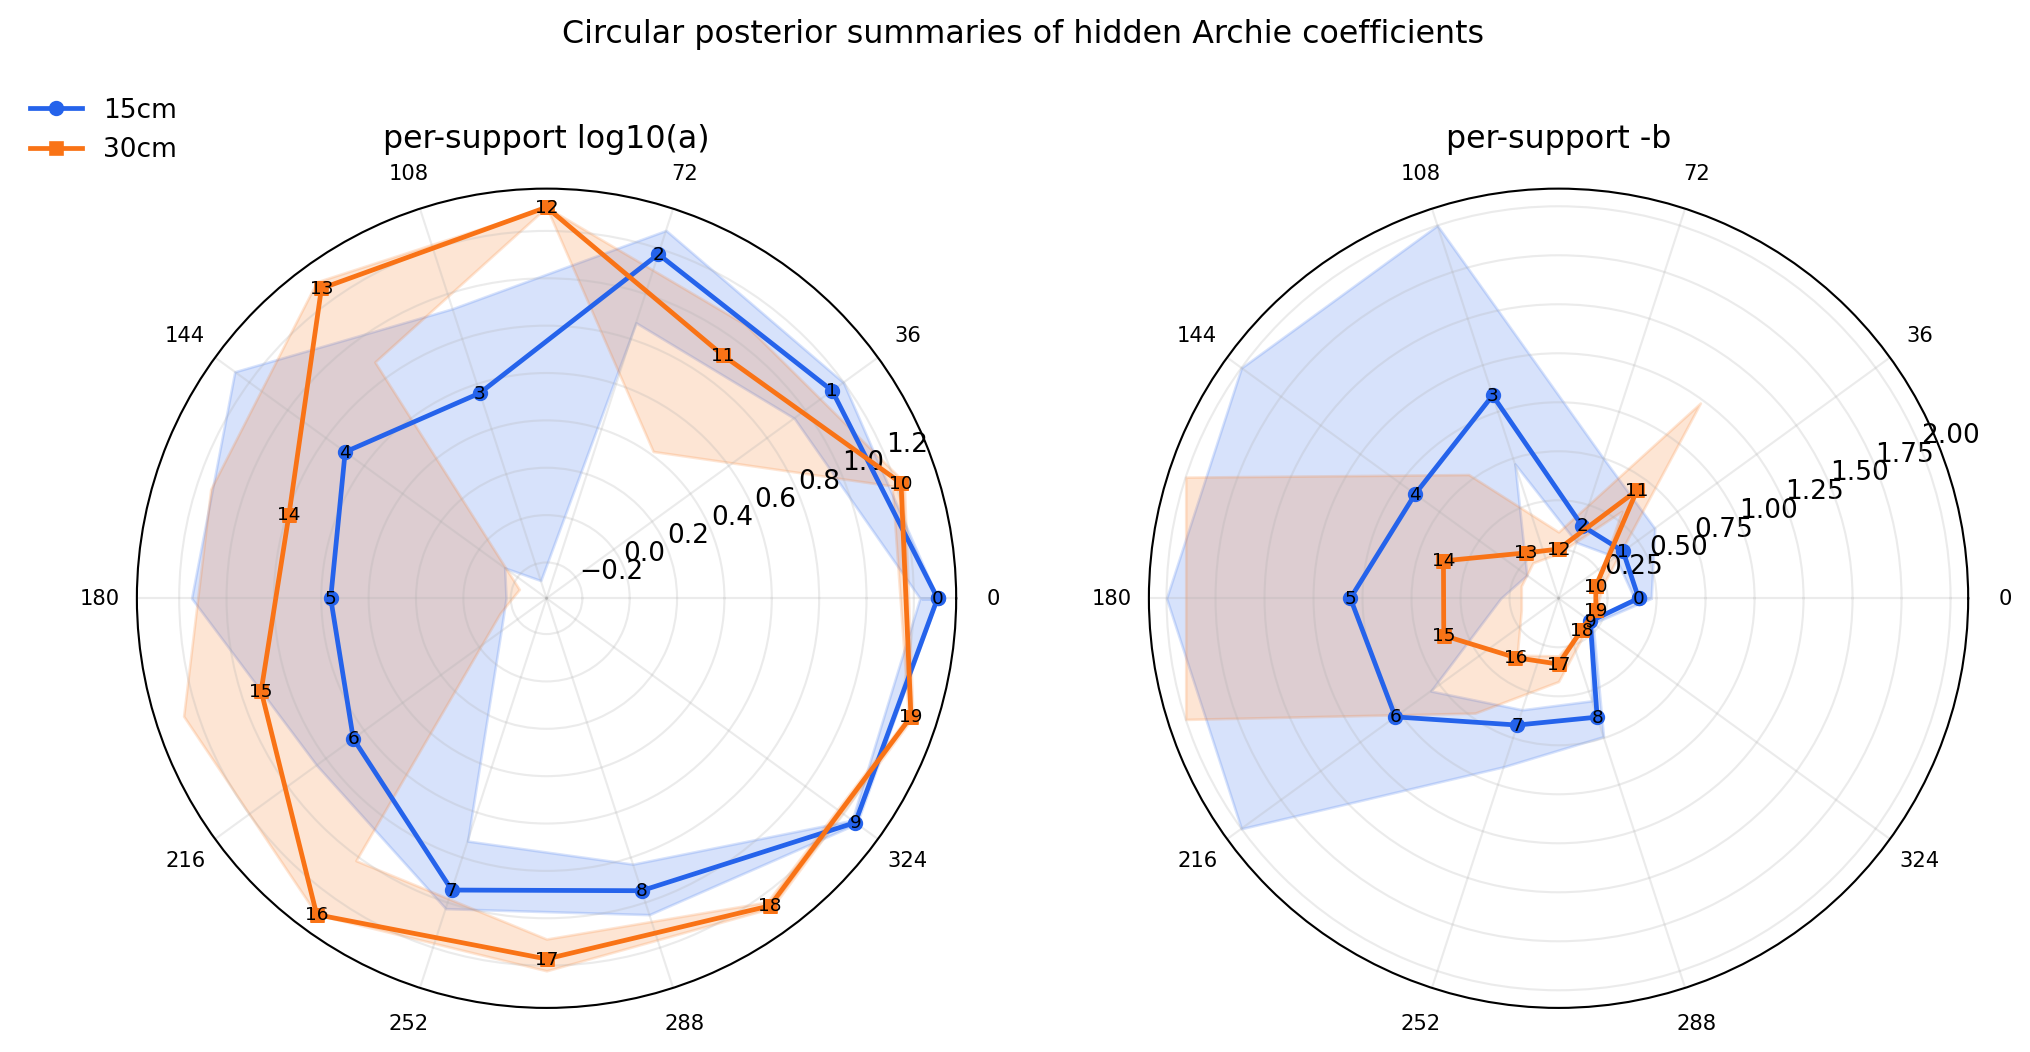
\includegraphics[width=0.98\textwidth]{resources/figures/numerical_archie_circular_posterior.png}
  \caption{Circular posterior summaries of local Archie coefficients.  Lines show
  posterior medians and shaded bands show 5--95\% intervals for the two ERT support
  rings.  Spatial structure in these nuisance coefficients is a measurement-model
  result, not a direct material-field result.}
  \label{fig:numerical-archie-circular-posterior}
\end{figure}

\FloatBarrier

\section{Permeability and Porosity Fields}
\label{sec:inversion-permeability-field}

The field result should be read as an ERT-conditioned material-field diagnostic.
Earlier permeability-magnitude examples showed that a spatial
\(\log_{10}K_{\mathrm{mag}}\) field improves the ERT response, but the best
current raw-\(\log_{10}\) fit uses both the permeability-magnitude field and the
bounded porosity field in Eqs.~\eqref{eq:permeability-magnitude-rf} and
\eqref{eq:porosity-kl-field}.  The parameterisation is therefore best described
as the minimal successful one seen in these files: scalar tensor orientation and
ratio, plus two random fields, \(K_{\mathrm{mag}}\) and \(\por\).  The available
results do not justify promoting a fully spatial tensor-random-field model as
better supported than this smaller parameterisation.

\begin{figure}[htbp]
  \centering
  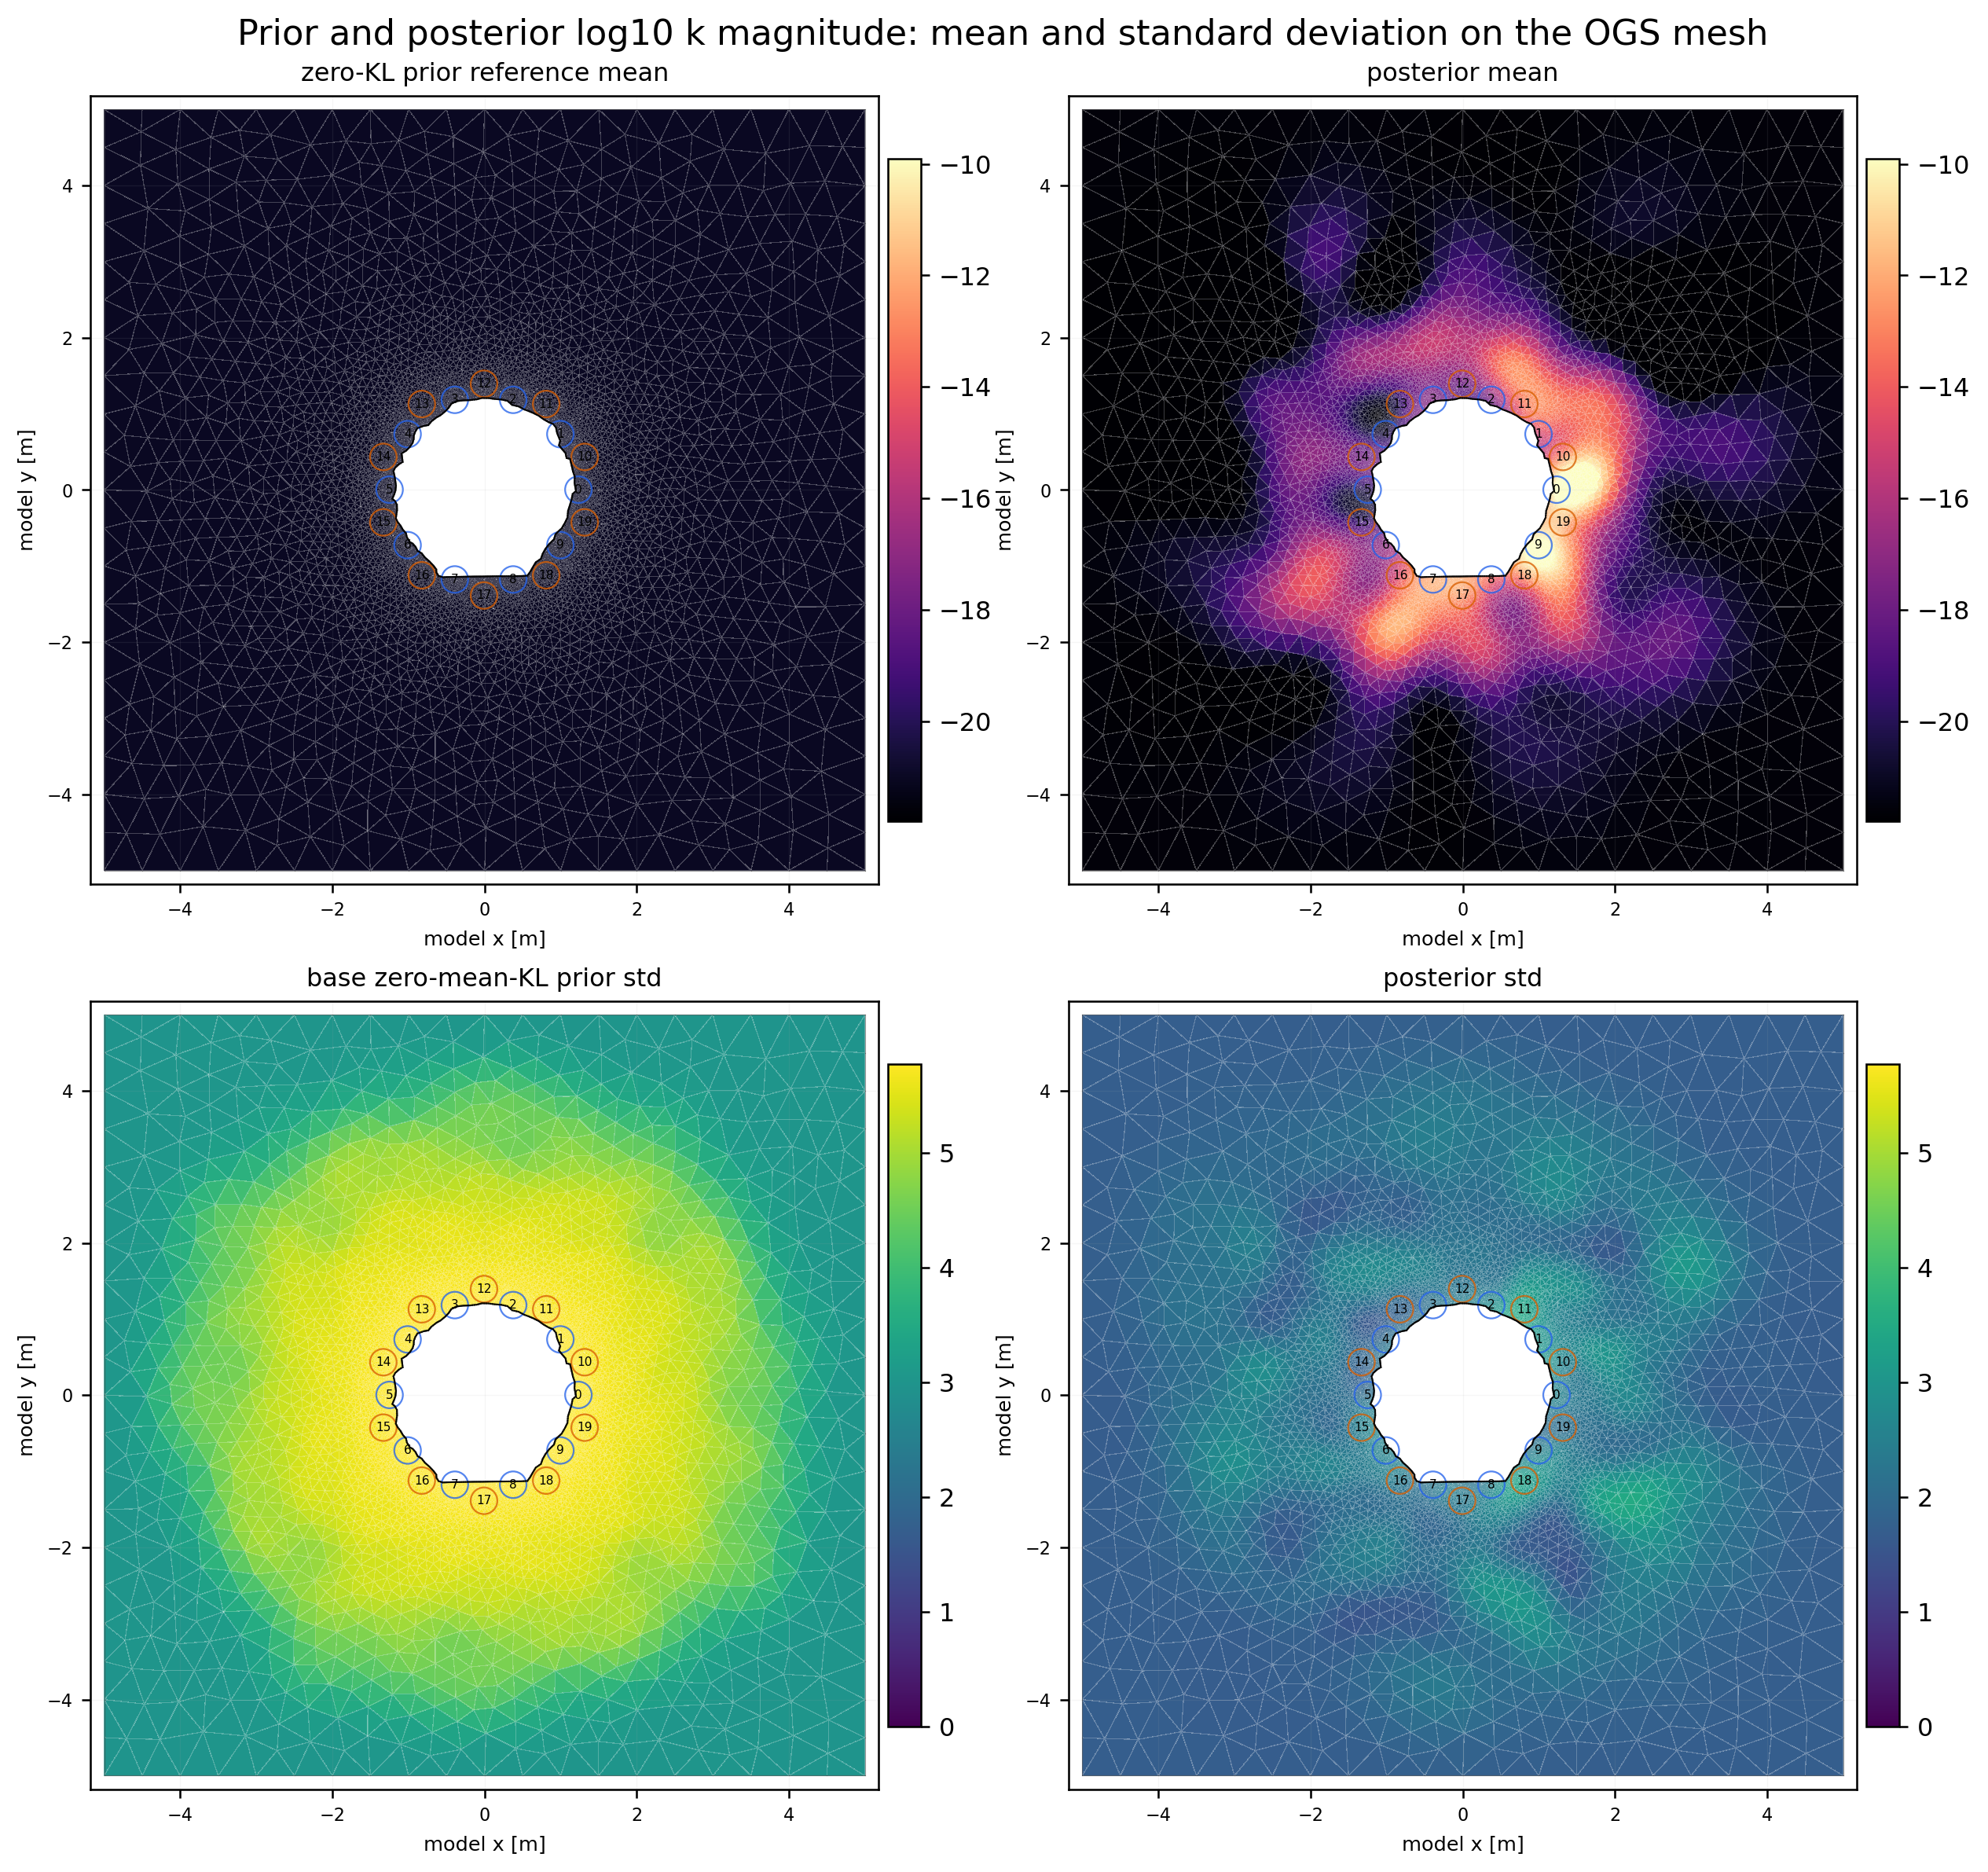
\includegraphics[width=0.96\textwidth]{resources/figures/numerical_permeability_magnitude_field.png}
  \caption{ERT-conditioned \(\log_{10}K_{\mathrm{mag}}\) field.  The figure compares
  the zero-KL prior reference and posterior summaries for permeability magnitude on
  the OGS mesh.}
  \label{fig:numerical-permeability-magnitude-field}
\end{figure}

In the retained posterior-field summary, the posterior mean
\(\log_{10}K_{\mathrm{mag}}\) field has spatial median \(-16.88\), 5--95\%
spatial range \(-21.66\) to \(-10.14\), and posterior standard-deviation median
\(2.31\).  These values show that ERT is pushing a broad permeability-magnitude
field, not a narrowly identified final map.

\begin{figure}[htbp]
  \centering
  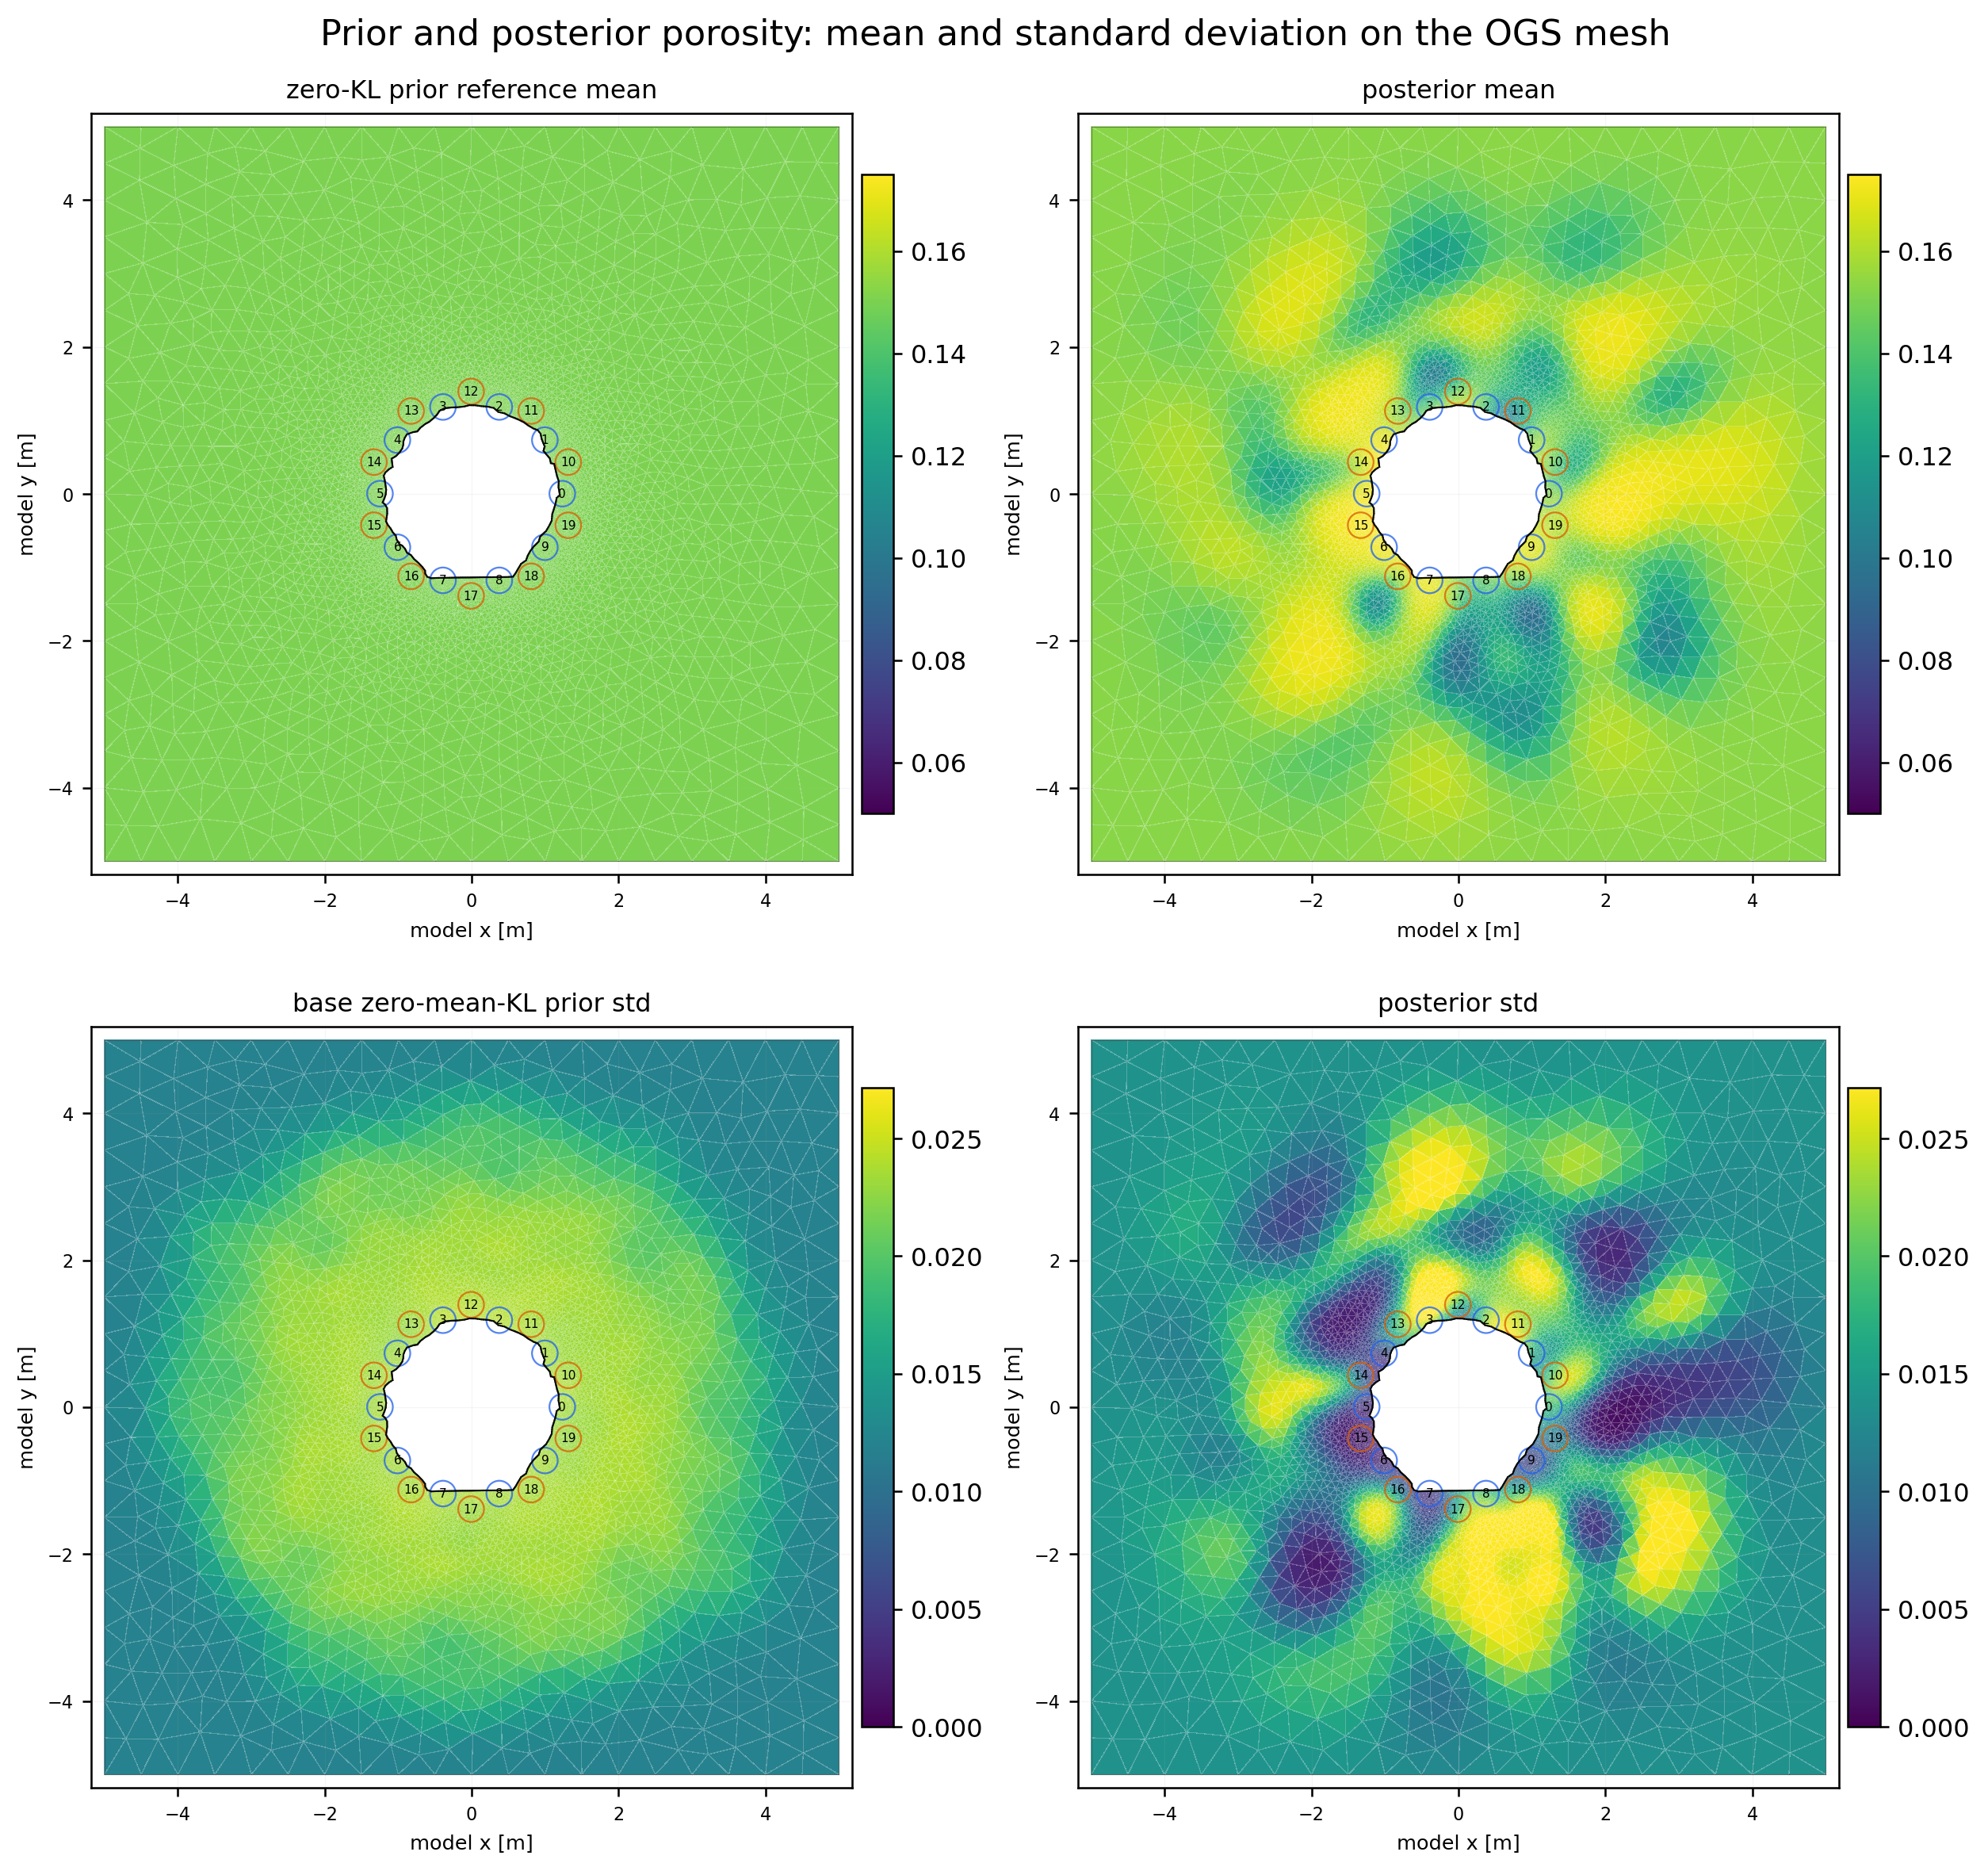
\includegraphics[width=0.96\textwidth]{resources/figures/numerical_porosity_field.png}
  \caption{ERT-conditioned porosity field.  The panels show the zero-KL
  prior-reference mean, posterior mean, base zero-mean-KL prior standard deviation,
  and posterior standard deviation on the native OGS mesh.}
  \label{fig:numerical-porosity-field}
\end{figure}

The porosity posterior is also spatially structured.  The posterior mean porosity
field has spatial median \(0.155\), 5--95\% spatial range \(0.119\)--\(0.172\),
and posterior standard-deviation median \(0.0147\).  This is not the fixed
\path{n_rd} porosity field from the base XML; it is an ERT-conditioned random-field
result and still needs exact-OGS checks and independent water-content or porosity
support before it becomes a released material field.

\begin{figure}[htbp]
  \centering
  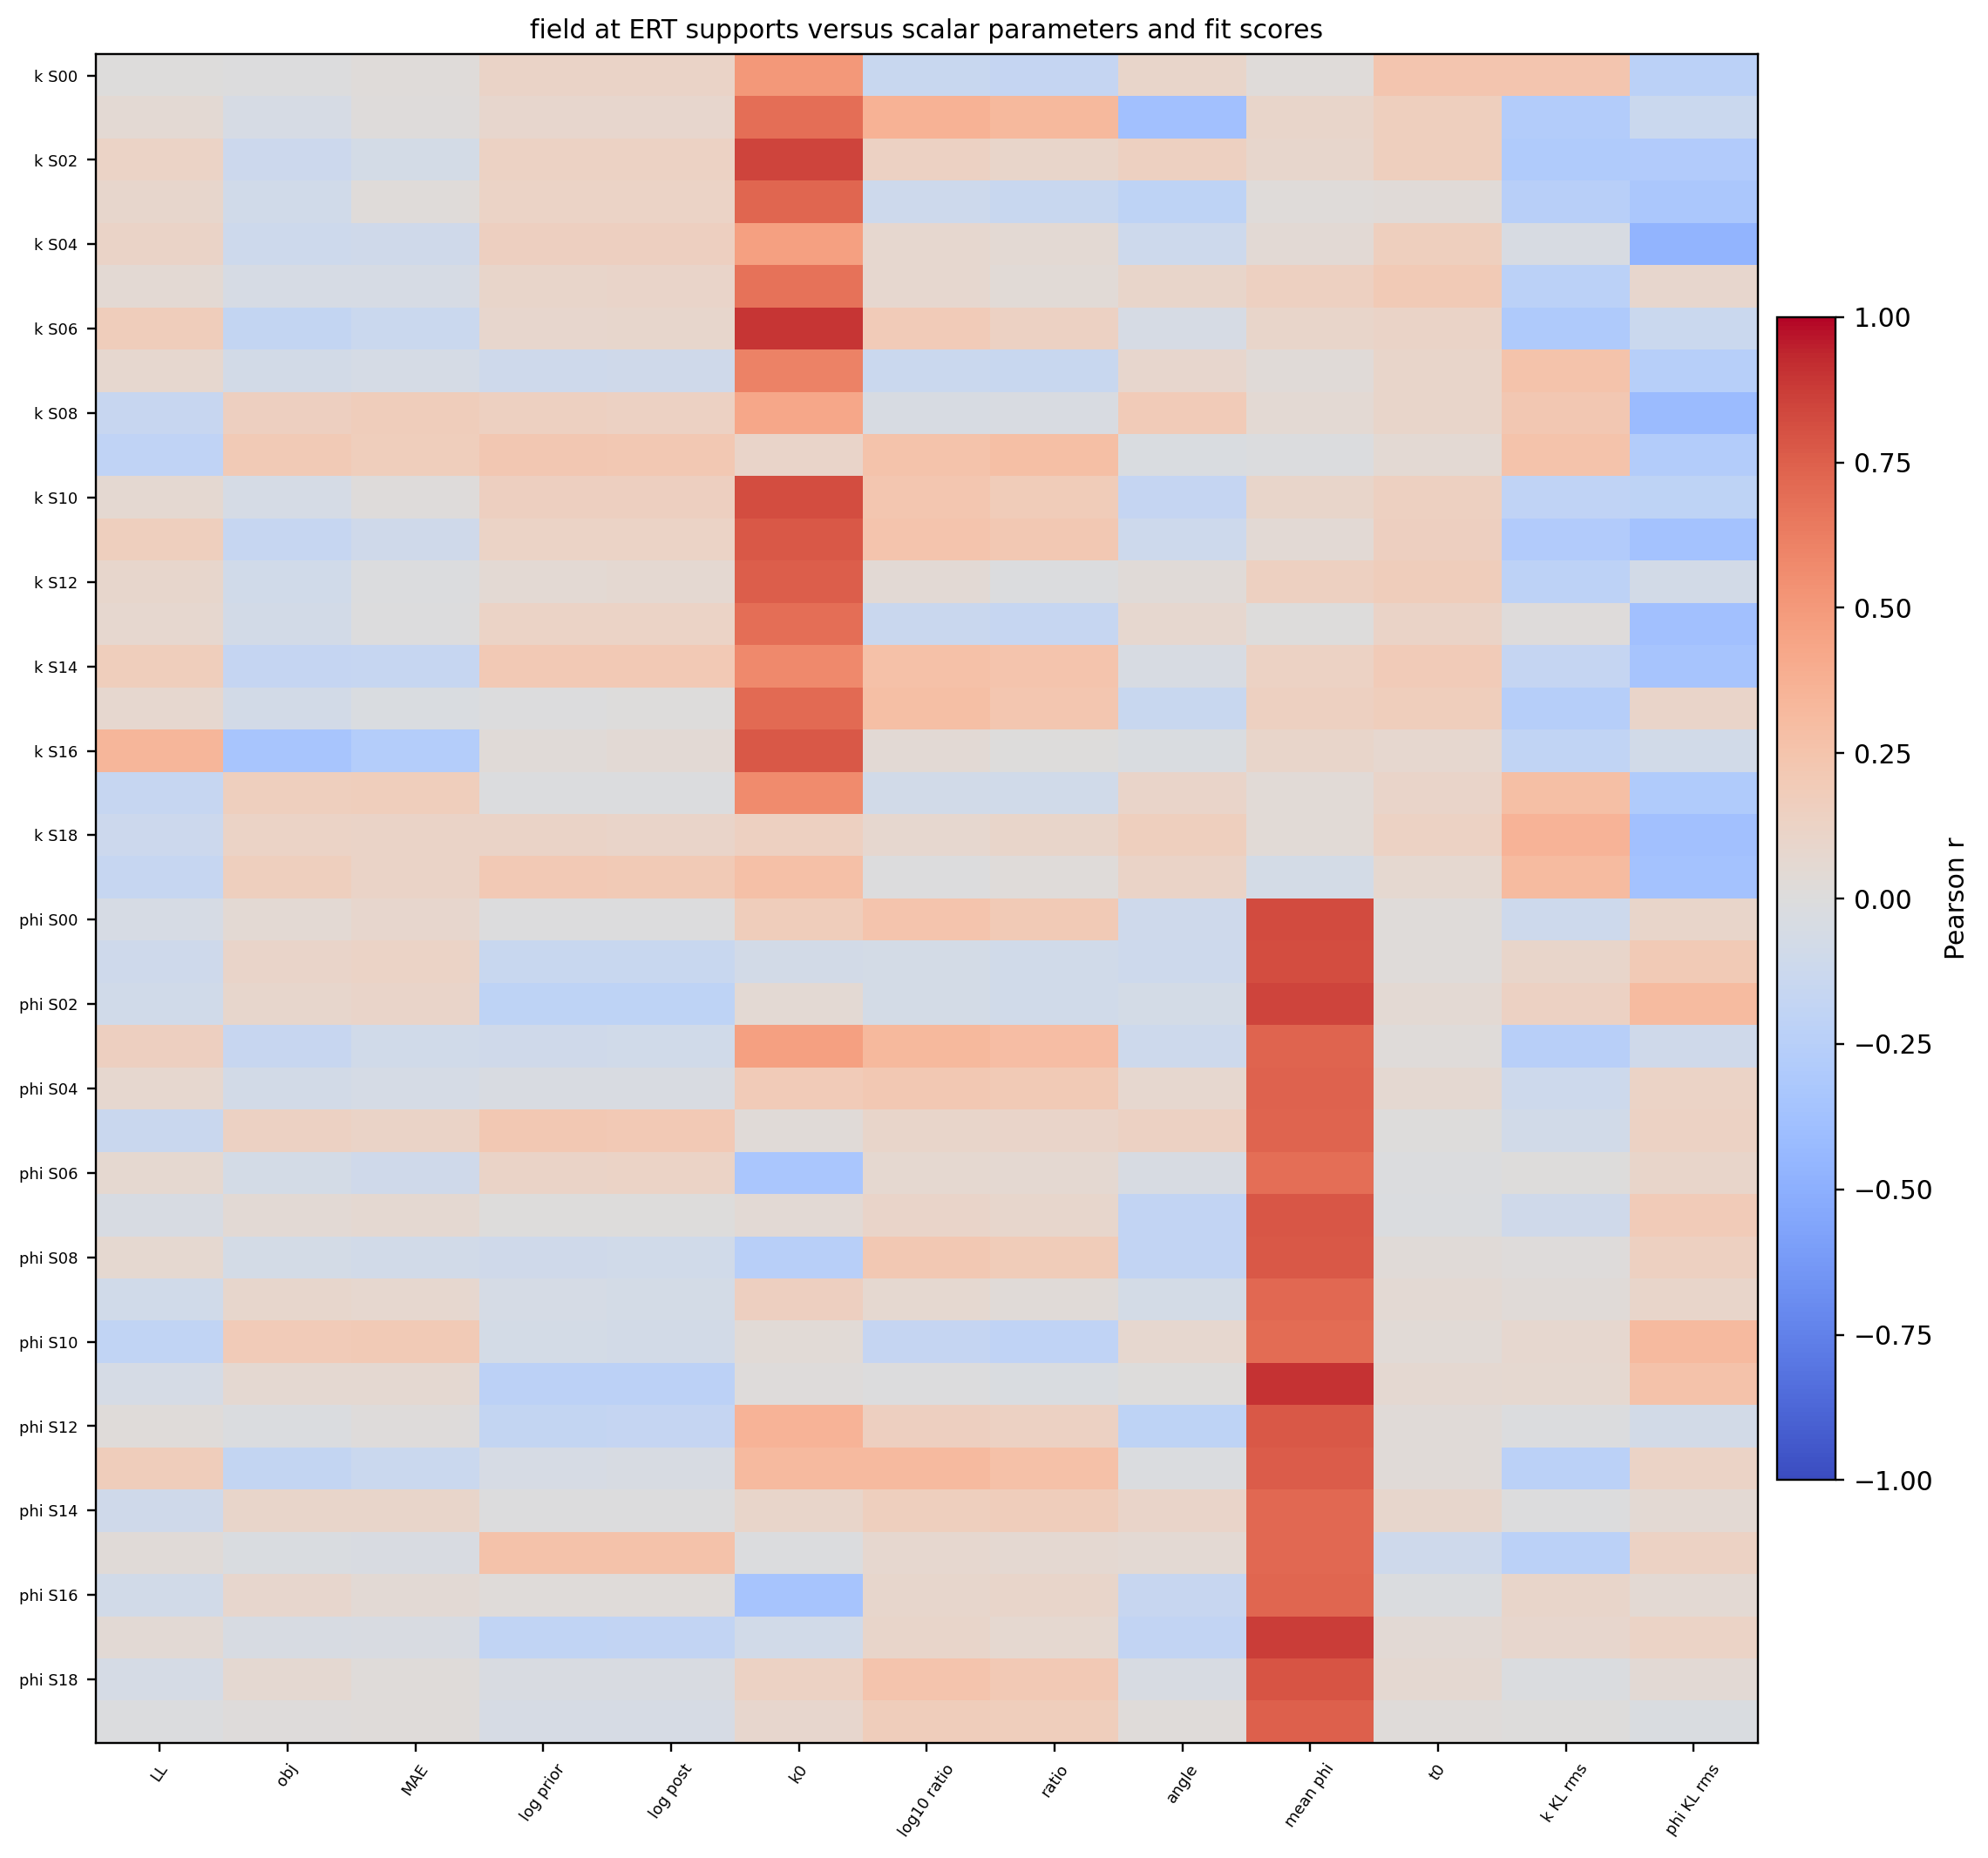
\includegraphics[width=0.98\textwidth]{resources/figures/numerical_support_field_scalar_correlations.png}
  \caption{Posterior correlations between ERT-support random-field values and scalar
  parameters or fit scores.  The permeability-support variables correlate most
  strongly with \(k_0\); porosity-support variables correlate most strongly with the
  mean porosity control.}
  \label{fig:numerical-support-field-scalar-correlations}
\end{figure}

\FloatBarrier

\section{Implications for the Rest of the Report}
\label{sec:inversion-implications}

The numerical examples move ERT from a future stream to a demonstrated calibration
target, but only within a narrow observation model: 20 ERT supports, 33 times,
an explicit time-alignment parameter, and Archie calibration.  They do not
assimilate NMR, Taupe/TDR, RH/suction, direct pressure, fractures, crackmeters,
levelling, or other hydro-mechanical streams.

The practical interpretation is therefore conservative.  Keep
\(K_{\mathrm{mag}}\) as the common permeability field written through
\path{k_i_rd}; use the porosity random field as an ERT-conditioned diagnostic until
it is checked by exact OGS and non-ERT evidence; and treat the local/global Archie
contrast as the main current ERT gate.  The next robust comparison should fix the
support mask, time-axis convention, covariance/down-weighting, and electrical
anisotropy treatment before turning these ERT-conditioned fields into a final
all-measurement material map.
